\section{\review{Magnetic Fields}}

% ============================================
%                Nomenclature
% ============================================
\subsection{\review{Nomenclature}}

Several notations coexist to denote magnetic fields. In this thesis, the
\textit{European Convention}~\cite{dilly_corrections_2022} is used for field indices, as shown
in \cref{tab:magnetic_fields:relation_indices}. MAD-X and MAD-NG, simulation softwares, however, use the
\textit{American Convention}. 

\begin{table}[H]
    \centering
    \begin{tabular}{lccc}
    \toprule
        Multipole     &     Index         &      MAD-X      \\
    \midrule                              
        Dipole        &     1             &     0           \\
        Quadrupole    &     2             &     1           \\
        Sextupole     &     3             &     2           \\
        Octupole      &     4             &     3           \\
        Decapole      &     5             &     4           \\
        Dodecapole    &     6             &     5           \\
        Decatetrapole &     7             &     6           \\
        Decahexapole  &     8             &     7           \\
    \bottomrule
    \end{tabular}
    \caption{Relation between the field indices used in this thesis and multipoles.}
    \label{tab:magnetic_fields:relation_indices}
  \end{table}

As such, unless explicitly stated, quantities such as the magnetic strength $b$ and normalized
strength $K$ presented latter will be expressed with the notation used in the first column. 
A schematic representation of magnets up to dodecapole, order 6, is given in
\cref{fig:background:magnetic_fields:schematics}.

\begin{figure}[!htb]
    \newlength{\magnetheight}
    \setlength{\magnetheight}{85px}
    \centering
    \begin{subfigure}{0.24\textwidth}
        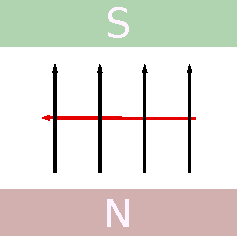
\includegraphics[height=\magnetheight]{images/magnets/dipole_normal.pdf}
        \caption{
           Normal Dipole 
        }
        \label{fig:MBNorm}
    \end{subfigure}
    %\begin{subfigure}{0.24\textwidth}
    %    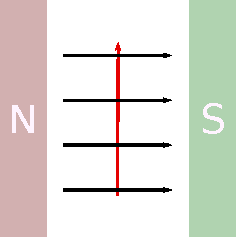
\includegraphics[height=\magnetheight]{images/magnets/dipole_skew.pdf}
    %    \caption{
    %       \Gls{skew} Dipole 
    %    }
    %    \label{fig:MBSkew}
    %\end{subfigure}
    \begin{subfigure}{0.243\textwidth}
        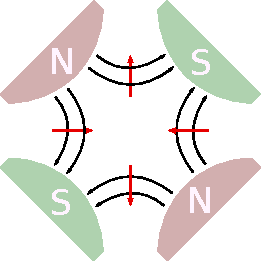
\includegraphics[height=\magnetheight]{images/magnets/quadrupole_normal_f.pdf}
        \caption{
           Normal Quadrupole 
        }
        \label{fig:MQNorm}
    \end{subfigure}
    %\begin{subfigure}{0.243\textwidth}
    %    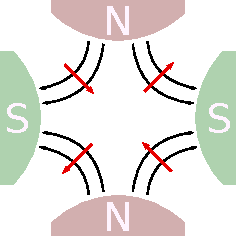
\includegraphics[height=\magnetheight]{images/magnets/quadrupole_skew.pdf}
    %    \caption{
    %       \Gls{skew} Quadrupole 
    %    }
    %    \label{fig:MQSkew}
    %\end{subfigure}
    \begin{subfigure}{0.243\textwidth}
        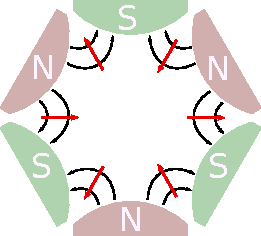
\includegraphics[height=\magnetheight]{images/magnets/sextupole_normal.pdf}
        \caption{
           Normal Sextupole 
        }
        \label{fig:MSNorm}
    \end{subfigure}
    \\
    \vspace{1em}
    %\begin{subfigure}{0.243\textwidth}
    %    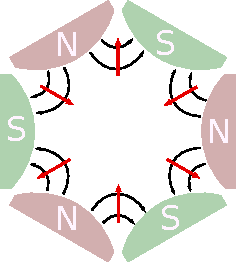
\includegraphics[height=\magnetheight]{images/magnets/sextupole_skew.pdf}
    %    \caption{
    %       \Gls{skew} Sextupole 
    %    }
    %    \label{fig:MSSkew}
    %\end{subfigure}
    \begin{subfigure}{0.243\textwidth}
        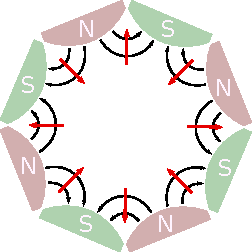
\includegraphics[height=\magnetheight]{images/magnets/octupole_normal.pdf}
        \caption{
           Normal Octupole 
        }
        \label{fig:MONorm}
    \end{subfigure}
    %\begin{subfigure}{0.243\textwidth}
    %    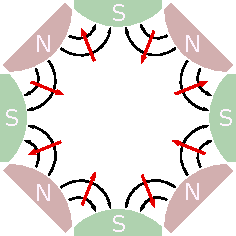
\includegraphics[height=\magnetheight]{images/magnets/octupole_skew.pdf}
    %    \caption{
    %       \Gls{skew} Octupole 
    %    }
    %    \label{fig:MOSkew}
    %\end{subfigure}
    \begin{subfigure}{0.243\textwidth}
        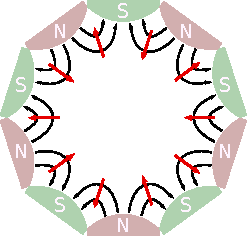
\includegraphics[height=\magnetheight]{images/magnets/decapole_normal.pdf}
        \caption{
           Normal Decapole 
        }
        \label{fig:MDNorm}
    \end{subfigure}
    %\begin{subfigure}{0.243\textwidth}
    %    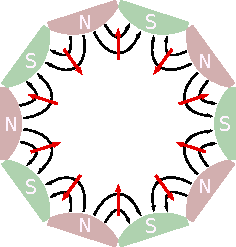
\includegraphics[height=\magnetheight]{images/magnets/decapole_skew.pdf}
    %    \caption{
    %       \Gls{skew} Decapole 
    %    }
    %    \label{fig:MDSkew}
    %\end{subfigure}
    \begin{subfigure}{0.243\textwidth}
        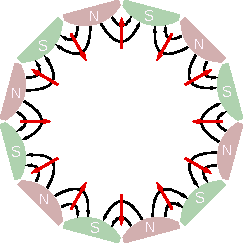
\includegraphics[height=\magnetheight]{images/magnets/dodecapole_normal.pdf}
        \caption{
           Normal Dodecapole 
        }
        \label{fig:MTNorm}
    \end{subfigure}
    %\begin{subfigure}{0.243\textwidth}
    %    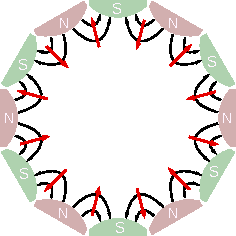
\includegraphics[height=\magnetheight]{images/magnets/dodecapole_skew.pdf}
    %    \caption{
    %       \Gls{skew} Dodecapole 
    %    }
    %    \label{fig:MTSkew}
    %\end{subfigure}
    \caption{
        Schematics of magnetic multipoles. In black the magnetic field lines,
        which extend also to the inner part of the magnets, 
        but drawing them there has been omitted for clarity of the figure.
        Red arrows indicate the direction of force on a 
        positive charge moving out of the page towards the reader.
        Courtesy of Joschua Dilly~\cite{dilly_corrections_2022}.
    }
    \label{fig:background:magnetic_fields:schematics}
\end{figure}



% ============================================
%              Multipole Expansion
% ============================================
\subsection{\review{Multipole Expansion}}

In order to force the particles to form a closed orbit, they are subjected to magnetic fields that
deflect their trajectories. The force exerted on a charged particle via electromagnetic fields is
the Lorentz force $\vec{F}$~\cite{wiedemann_particle_2015},

\begin{equation}
    \vec{F} = \frac{\diff \vec{p}}{\diff t} = q \left( \vec{E} + \vec{v} \times \vec{B} \right),
\end{equation}

where $\vec{p}$ is the momentum of the particle, $q$ its charge, $\vec{v}$ its charge, $\vec{E}$ the
electric field and $\vec{B}$ the magnetic field. With particles close to the speed of light, it
becomes apparent that magnetic fields are dominant in the resulting force and are thus used to act
on the particles trajectories.
The guiding magnetic field in the transverse planes \textit{x} and \textit{y} can be described using
a \textit{multipole expansion}, where the components of the magnetic field can be written as a
series of terms corresponding to different orders of multipoles. The multipole expansion is then
given in terms of the normal and skew field gradients $\mathcal{B}$ and $\mathcal{A}$ with
multipoles of order $n$~\cite{wolf_engineering_2001},
\begin{equation}
    B_y + iB_x = \sum_{n=1}^\infty \left(\mathcal{B}_n + i\mathcal{A}_n \right)  (x+iy)^{n-1}.
\end{equation}

The normal and skew field gradients $\mathcal{B}$ and $\mathcal{A}$ for a multipole of order $n$ can
then be calculated from this complex field,

\begin{equation}
    \mathcal{B}_n + i\mathcal{A}_n = \left.\frac{1}{(n-1)!} \cdot \frac{\partial^{n-1}\left(B_y + iB_x\right)}{\partial(x+iy)^{n-1}}\right|_{x=0,y=0}.
\end{equation}

Expanded up to octupoles, the magnetic field acting on the horizontal plane reads,

\begin{equation}
    B_y = \underbrace{B_{y0}}_{\textrm{dipole}}
        + \underbrace{\frac{\partial B_y}{\partial x} \cdot x}_{\textrm{quadrupole}}
        + \underbrace{\frac{1}{2!} \frac{\partial^2 B_y}{\partial x^2} \cdot x^2}_{\textrm{sextupole}}
        + \underbrace{\frac{1}{3!} \frac{\partial^3 B_y}{\partial x^3} \cdot x^3}_{\textrm{octupole}}
        + \cdots
\end{equation}

An ideal magnet would  often produce either a sole normal or skew field. However, this is not
applicable to real-life magnets that are imperfect, due to design and manufacturing constraints.
Field errors are thus introduced, relative to the main field of the ideal 2N-pole magnet at a
reference radius $r_{ref}$, as shown in \cref{eq:magnetic_field:relative_errors}. The coefficients
of the normal and skew relative field errors, referred to as $a_n$ and $b_n$, are dimensionless but
often given in \textit{units} of $10^{-4}$.

\begin{equation}
    B_y + iB_x = 
        \begin{cases}
            \mathcal{B}_N \cdot \sum_{n+1}^\infty (b_n + ia_n) \left(\frac{x+iy}{r_{ref}}\right)^{n-1}\text{, for normal magnets}\\
            \mathcal{A}_N \cdot \sum_{n+1}^\infty (b_n + ia_n) \left(\frac{x+iy}{r_{ref}}\right)^{n-1}\text{, for skew magnets}
        \end{cases}
    \label{eq:magnetic_field:relative_errors}
\end{equation}

The total normal and skew field components of order $n$ for an imperfect 2N-pole magnet is thus
given by the following equation:

\begin{equation}
    \begin{aligned}
        \mathcal{B}_n &= \mathcal{B}_N \cdot \frac{b_n}{r_{ref}^{n-1}}, \\
        \mathcal{A}_n &= \mathcal{A}_N \cdot \frac{a_n}{r_{ref}^{n-1}}.
    \end{aligned}
\end{equation}

The unit of the field is relative to the multipole order $n$: $[\text{Tm}^{1-n}]$.



% ============================================
%              Normalization
% ============================================
\subsection{\review{Beam Rigidity and Normalization}}

\subsubsection{\review{Beam Rigidity}}

In order to bend particles to form a ring, the force acting on the particles given by the Lorentz
force must be equal to the centrifugal force~\cite{holzer_design_2020,wiedemann_particle_2015}:

\begin{equation}
    q(\vec{E} + \vec{v} \times \vec{B}) = \frac{mv^2}{\rho},
\end{equation}

with $q$ the charge of the particle, $\vec{E}$ and $\vec{B}$ respectively the electric and magnetic
field strengths, $\vec{v}$ the velocity of the particle, $m$ its mass and $\rho$ the radius of the
circular path. 
The beam rigidity is a quantification of the ability of a magnetic field to bend the trajectory of a
particle. It is derived from the previous equation and relates the
magnetic field $B$, the radius of curvature $\rho$ to the momentum $p$ and charge $q$ of the
particle. By neglecting the electrical force and using $p = mv$,

\begin{equation}
    \begin{aligned}
                           & qvB &&= \frac{mv^2}{\rho}, \\
        \rightarrow  \quad & qB &&= \frac{p}{\rho}, \\
        \rightarrow  \quad & B\rho \quad [\textrm{T.m}] &&= \frac{p}{q}.
    \end{aligned}
    \label{eq:magnetic_fields_beam_rigidity}
\end{equation}

The beam rigidity can also be expressed via the momentum in GeV. The usual approximation is then
given by,

\begin{equation}
    B \rho \approx 3.33 \cdot pc.
\end{equation}

This quantity is of interest when designing an accelerator to set the maximum field as well as the required
radius of curvature for a specific momentum and particle.
An interesting metric of an accelerator is also its \textit{filling factor}, or percentage of
dipoles in the machine. It can be calculated via the radius of curvature: $f = \rho / r$. A low 
filling factors means more space for other magnets, collimators, beam instrumentation, etc.

\subsubsection{\review{Field Normalization}}

The Beam Rigidity is also used as a way to normalize magnetic field strengths in particle
accelerators where the momentum of the particle changes (i.e. acceleration or deceleration).
The normalized Normal and Skew magnetic strengths $K$ and $J$ for a multipole of order $n$ are thus
given by~\cite{wolf_engineering_2001} the following,

\begin{equation}
    \begin{aligned}
        K_n =  \frac{q}{p} &(n-1)! \mathcal{B}_n, \\ 
        J_n =  \frac{q}{p} &(n-1)! \mathcal{A}_n,
    \end{aligned}
    \label{eq:magnetic_fields_normalized}
\end{equation}

with $p$ the momentum of the particle, $q$ its charge and $\mathcal{B}$ and $\mathcal{A}$ the field
gradients.


% ============================================
%            Hamiltonian Dynamics
% ============================================
\subsection{\review{Hamiltonian}}

The Hamiltonian describing the motion of relativistic particles in static electromagnetic fields is
given by~\cite{wolski_beam_2014},
\begin{equation}
    H = c \sqrt{(\mathbf{p}-q\mathbf{A})^2 + m^2c^2} + q\phi.
\end{equation}

where $\phi$ is the scalar potential, $\mathbf{A}$ the vector potential, $q$, $\mathbf{p}$ and $m$
respectively the charge, canonical momentum and mass of the particle and $c$ the celerity of light.

After having changed this Hamiltonian to be dependent on curved coordinates, introduced in the next
section, the motion in the transverse planes for a given multipole of order $n$ (other than dipoles)
can be described by the following~\cite{wolski_beam_2014},

\begin{equation}
    \begin{aligned}
        H &= \frac{q}{p} \Re \left[ \sum_{n>1} (\mathcal{B}_n + i\mathcal{A}_n) \frac{(x+iy)^n}{n} \right] \\
          &= \Re \left[ \sum_{n>1} (K_n + iJ_n) \frac{(x+iy)^n}{n!} \right].
    \end{aligned}
    \label{eq:hamiltonian_magnet}
\end{equation}

Quite often, when studying the effect of a magnet on the beam, only one component is required, and
the sum can thus be dropped.
The normal and skew fields can also be isolated in order to consider their sole effect as shown
in the following,

\begin{equation}
    \begin{aligned}
        N_n &=  &&\frac{1}{n!} K_n \Re \left[ (x+iy)^n \right], \\
        S_n &= -&&\frac{1}{n!} J_n \Im \left[ (x+iy)^n \right].
    \end{aligned}
    \label{eq:normal_skew_hamiltonian_magnet}
\end{equation}



% ============================================
%                 Harmonics
% ============================================
\subsection{\review{Harmonics}}
The magnetic fields in the LHC are generated by the coils of its magnets. However, real-world
magnets never produce a perfect, single field as desired. Instead, some field errors, known as
\textit{allowed harmonics}, naturally arise due to the geometric symmetries of the coils. As a
result, the main dipoles of the LHC can generate fields resembling those of sextupoles, decapoles,
decatetrapoles, and so on~\cite{deniau_magnetic_2009}. Additionally, manufacturing imperfections
contribute to field errors beyond the allowed ones, an example being octupolar errors seen in
the LHC dipoles.

During the design of the LHC, the main dipoles have been identified to generate significant field
errors. Magnetic measurements of those various fields were thus taken and magnetic tables built
based on real-life magnets nowadays installed in the machine. Those magnetic tables, computed for
each LHC configuration by \textit{WISE}~\cite{p_hagen_wise_2006} are used by simulation softwares.
Predictions of field errors and compensating strength for the correctors is computed by the Field
Description for the LHC (\textit{FiDeL}, \cite{noauthor_fidel_2021}). FiDeL is used in the LHC
control system in operation to compensate the field errors depending on the current configuration of
the machine.

\begin{figure}[!htb]
    \centering
    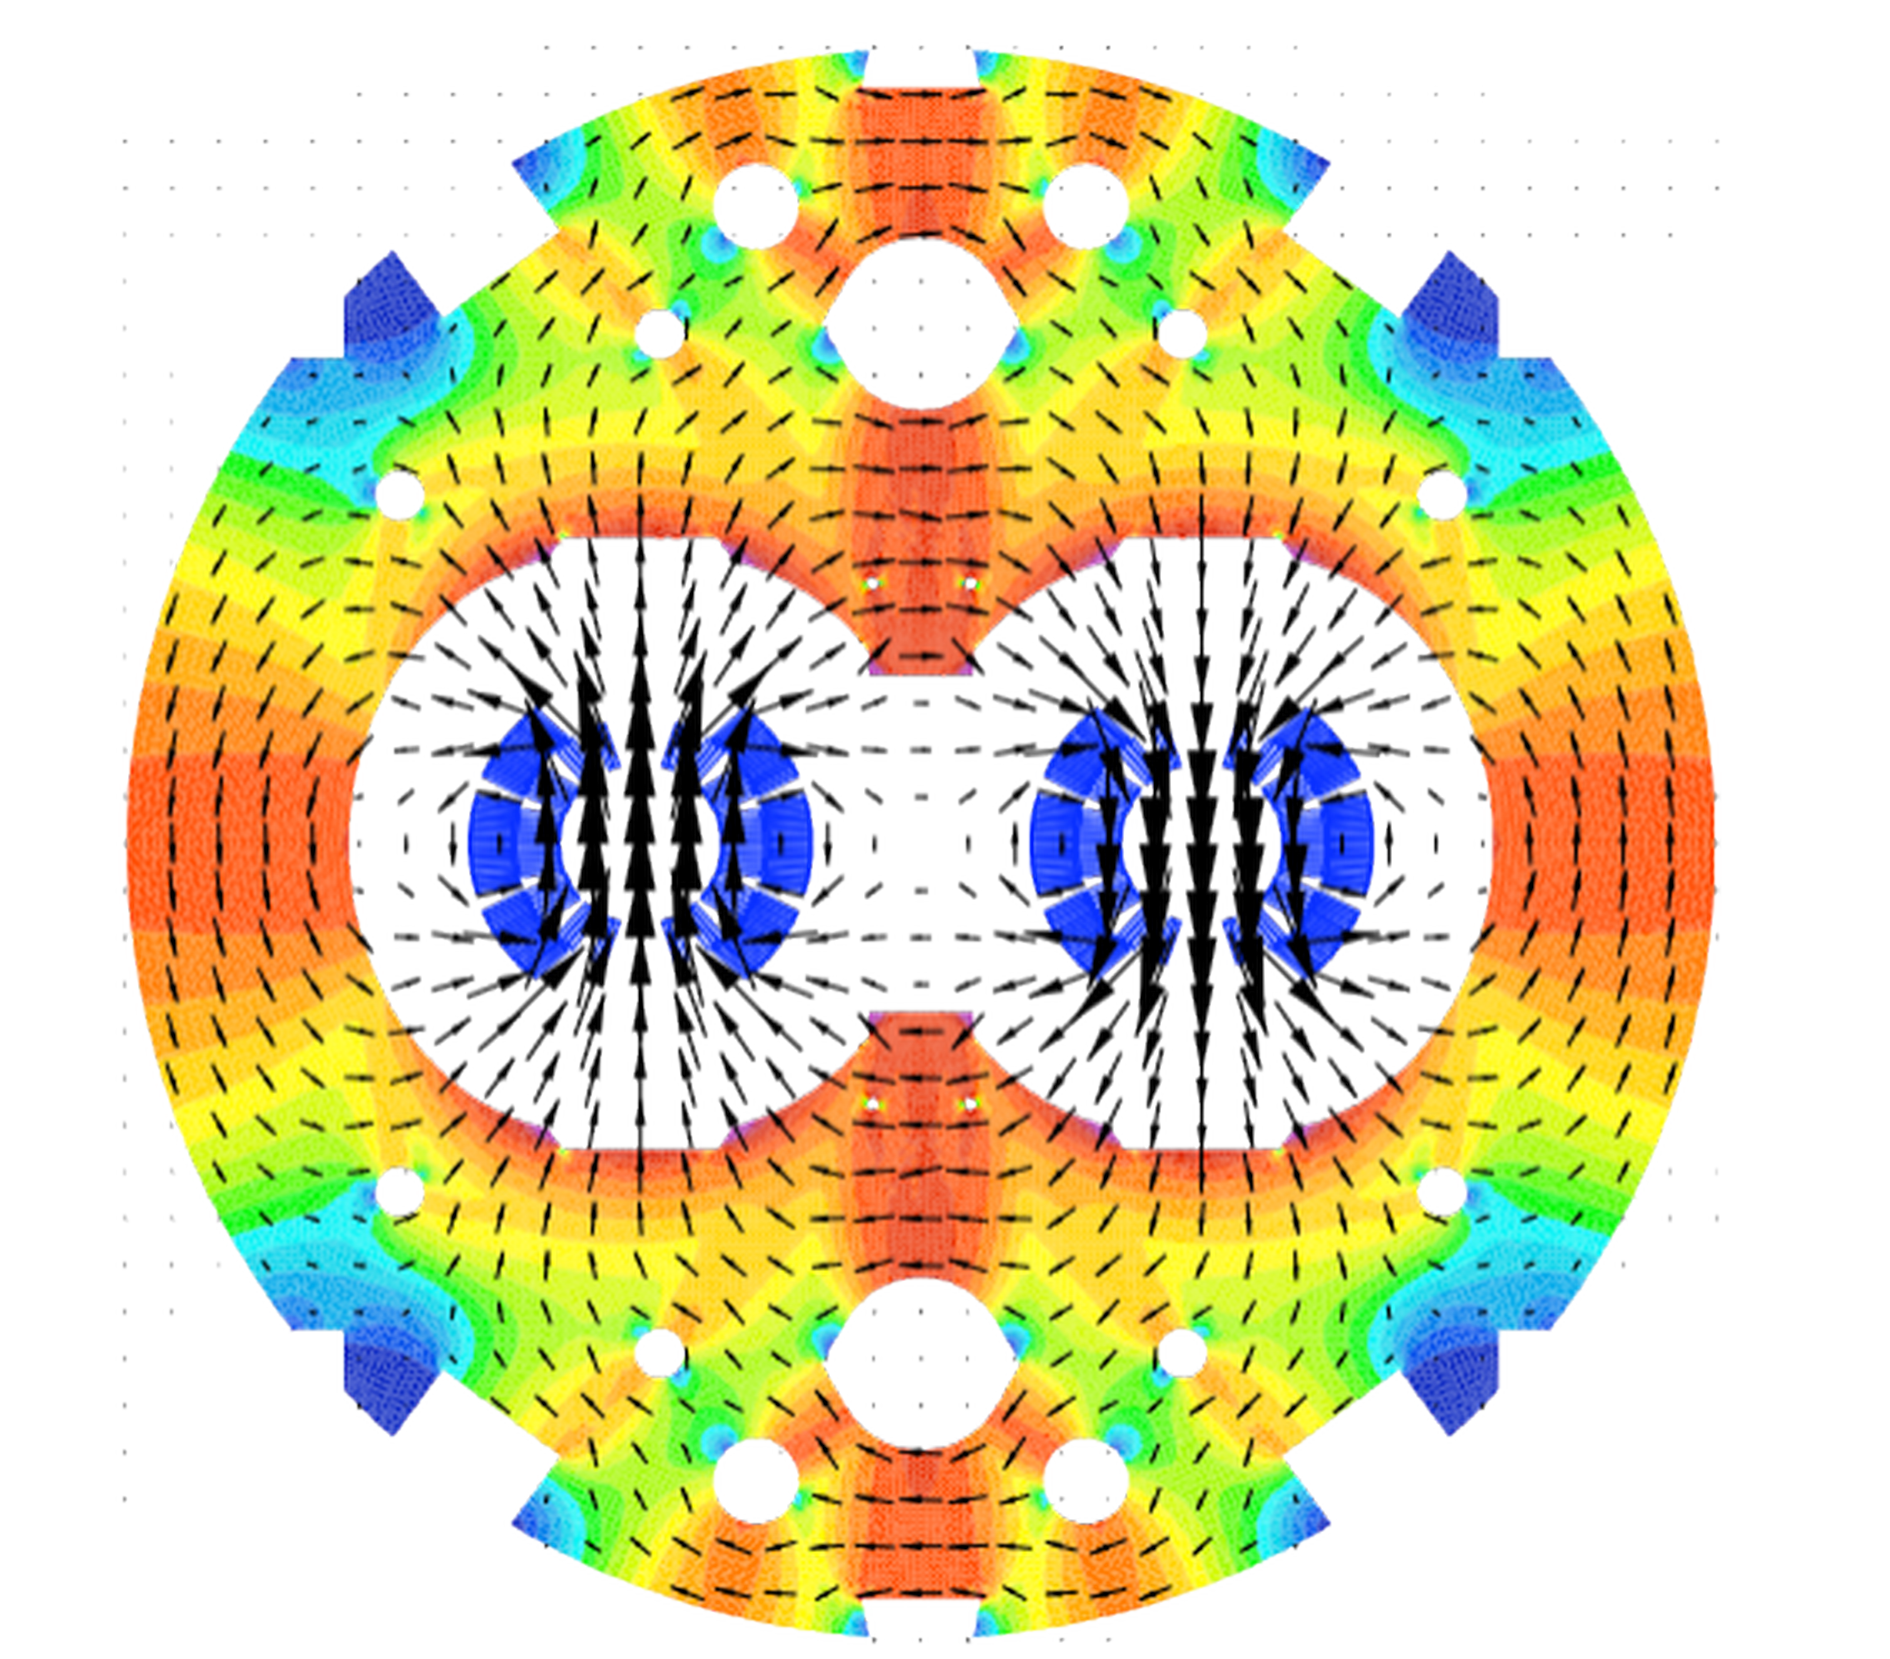
\includegraphics[width=0.4\textwidth]{./images/main_dipole_fields.png}
    \caption{Magnetic field in a dipole magnet~\cite{deniau_magnetic_2009}.}
    \label{fig:decapoles:magnetic_field_dipole}
\end{figure}

\FloatBarrier
